В данном документе представлена спецификация ЯЗ, который 
является языком запросов к объектной модели. %~\cite{ODMG_3}. 
ЯЗ представляет собой экспериментальную платформу для исследований в области
взаимодействия объектно-ориентированных систем и систем баз данных (БД).

Основной целью ЯЗ является решение следующих проблем:
\begin{enumerate}
    \item упрощение языка запросов, но сохранение при этом всех возможностей
    OQL\footnote{Многие из которых достались ему в наследство от SQL.} для объектных БД;
    \item возможность с помощью ЯЗ выполнять преобразования
данных из БД в форму, которая требуется пользователю.
\end{enumerate}

Также существует реализация ЯЗ, выполненная  
для виртуальной машины JVM (ЯЗ4J) на основе Criteria API 2.0. %~\cite{JPA_2}. 
В некоторых случаях когда решение по
механизму обеспечения возможности возлагается на реализацию ЯЗ, 
в качестве примера того, как это может быть сделано, будет приводиться реализация для JVM.

Для демонстрации возможностей и разъяснения особенностей ЯЗ будут приводиться
примеры на объектной модели
\footnote{Внутреннюю структуру классов см. в приложении~\ref{son_code}}, представленной на рис.~\ref{fig:son-model}.

\begin{figure}[hbt]
  \centering
  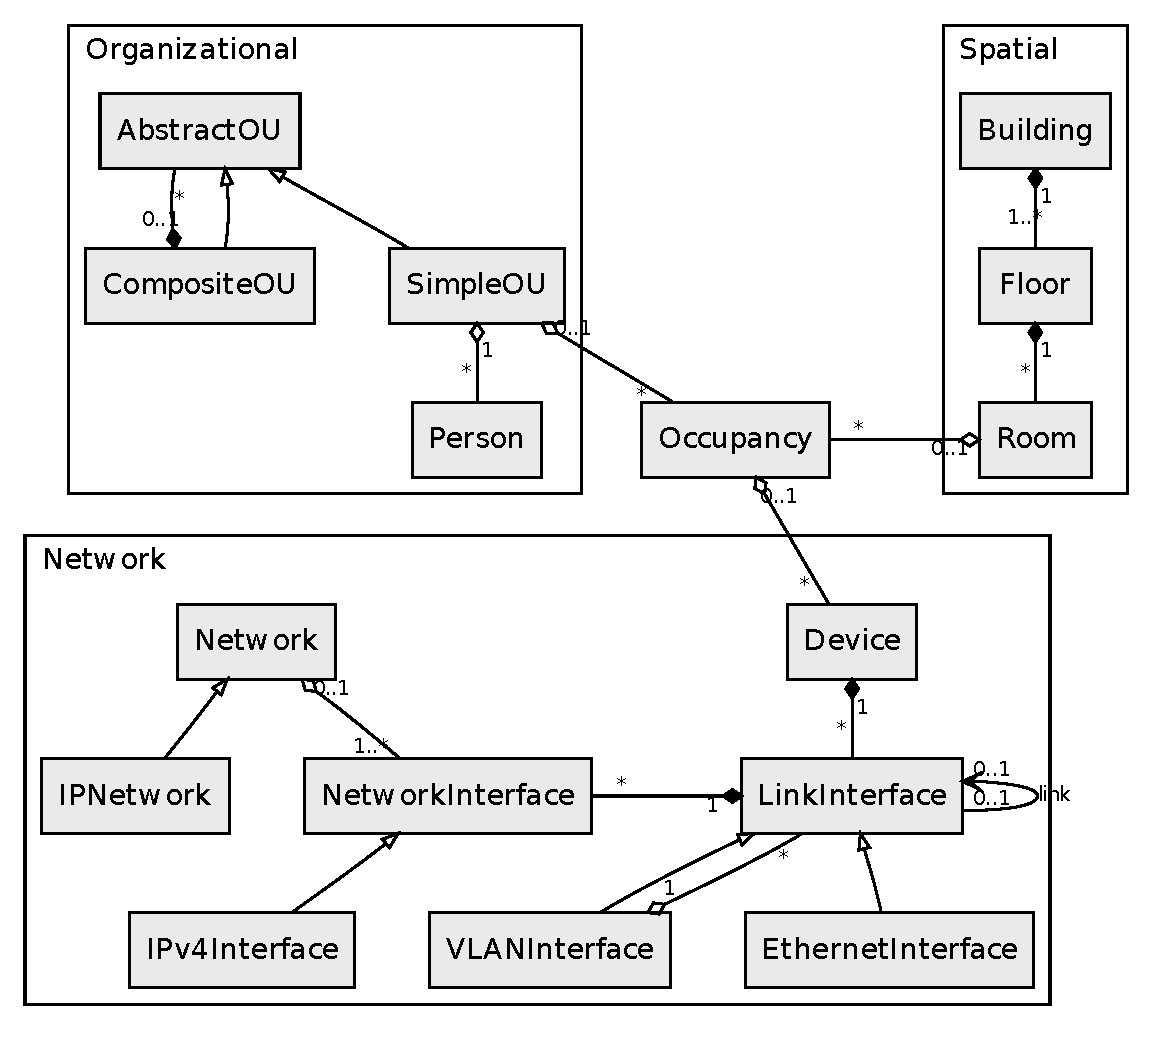
\includegraphics[scale=0.7]{figures/son}
  \caption{Пример объектной модели.}%~\cite{MS-Kryshen2008}.}
  \label{fig:son-model}
\end{figure}

%Псевдокод классов данной модели см. в приложении~\ref{son_code}.

Полное формальное описание языка в форме Бэкуса-Наура см. в приложении~\ref{oqlite_bnf}.




\subsection{Стиль документа}
Запросы в тексте будут выноситься на отдельную строку и для их написания
будет использоваться полужирный курсив: 
\query{device.building.name=``ГК''}

Если необходимо, то будет дана расшифровка ЯЗ-запроса на естественном языке. В таком случае
запрос будет выглядеть следующим образом:
\queryexpl{Найти все устройства в здании главного корпуса}{device.building.name=``ГК''}

Для названий классов или свойств классов, а также имен функций в тексте будет использоваться
\cl{курсив}.
